\section{Static System}
\subsection{Overview and Software}
To test our ideas, we developed a hardware prototype of a monocular near-eye display and implemented an offline version of our proposed rendering pipeline. The offline rendering pipeline begins with the rendering of a virtual scene using OpenGL/GLSL to generate an RGB image and a linearized 16-bit depth map of the virtual scene. The RGB image and depth map are processed in MATLAB to generate a series of binary images and RGB LED brightness values. The binary images are uploaded to and displayed by the DMD controller, and the RGB LED brightness values are used by a custom RGB LED driver for precise high-speed control over each LED's brightness. An ARM-based microcontroller provides synchronization between the lens, the DMD controller, and the custom RGB LED driver. Below we discuss each hardware component in detail.

\begin{figure}[t]
\centering
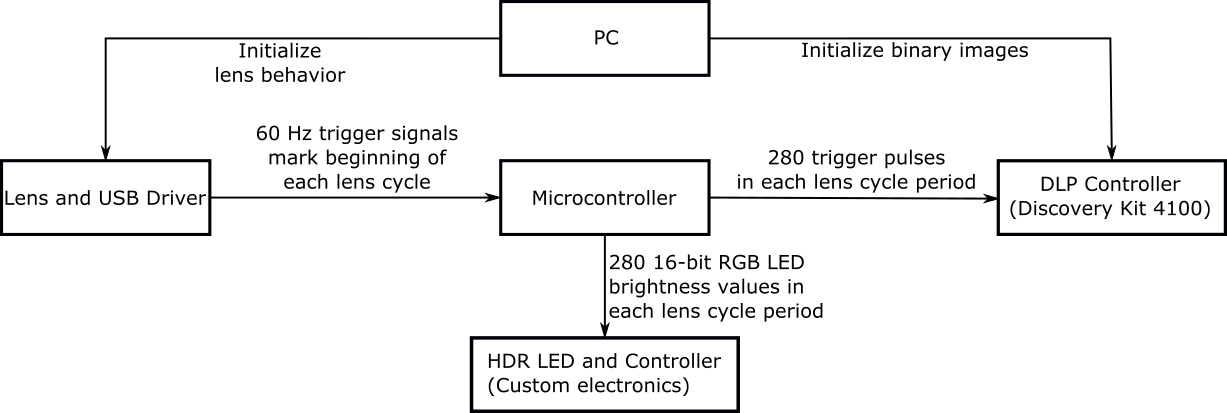
\includegraphics[width=\columnwidth]{images/volumetric/blockdiagram-timing}
\caption[Volumetric NED: overview of display components and timing relations]{Diagram shows the various hardware components and their timing relations to each other in the display's operational state.}
\label{fig:volumetric:blockdiagram-timing}
\end{figure}



\subsection{Hardware}
\paragraph{Focus-tunable Lens} The focus-tunable lens used is the Optotune EL-10-30-TC-VIS. The optical power of the lens is controlled via a manufacturer-provided software and a USB-connected lens driver. The optical power can be set to a static value, or it can be set to follow a rectangular, sinusoidal, or triangular signal for a wide range of frequencies (0.25 Hz to 2000 Hz). For this chapter, all experiments were conducted with the optical power of the lens configured to follow a triangular signal of 60 Hz frequency, and the maximum and minimum lens powers of the triangular signal were approximately 50$m^{-1}$ and 120$m^{-1}$. 

\begin{figure}[tb!]
\centering
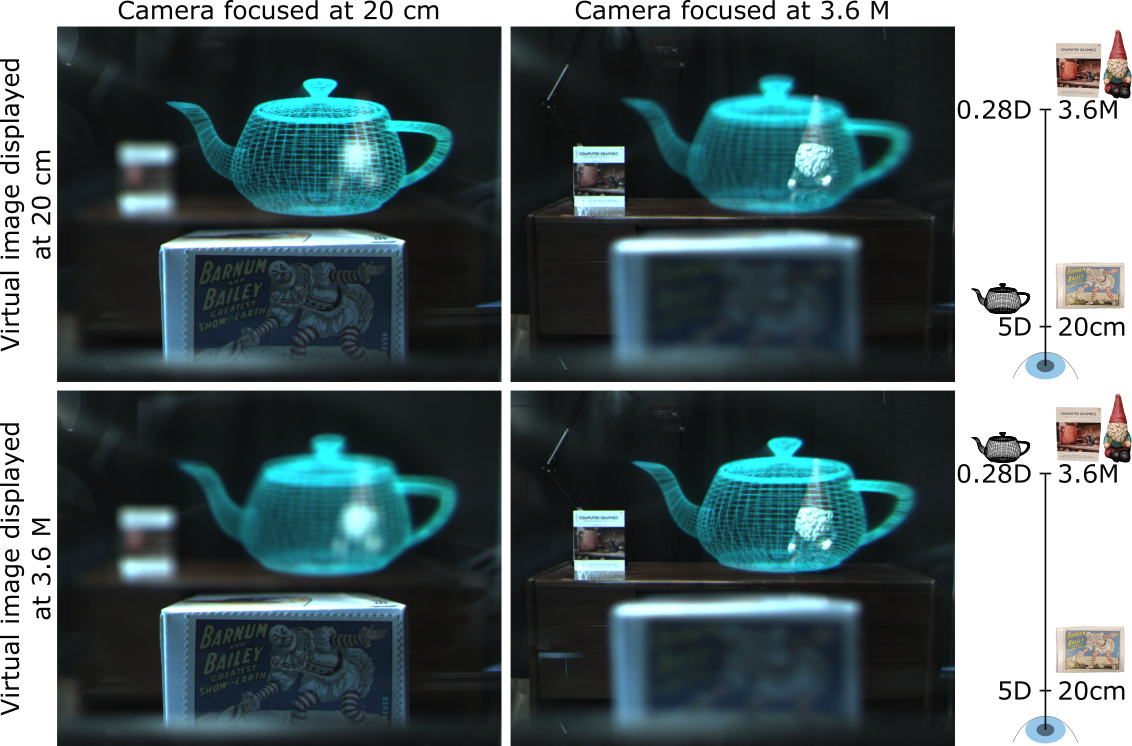
\includegraphics[width=\columnwidth]{images/volumetric/single_plane_images}
\caption[Volumetric NED: Examples of individual depth planes]{View through our near-eye display when only one out of the 280 binary image planes is encoded with a binary image. This figure gives an idea of how each binary image is perceived by an eye or a camera. When all binary images are encoded with appropriate content, a time-integrated color volume occupying a large depth range can be seen (see Figure~\ref{fig:volumetric:results}).}
\label{fig:volumetric:single_plane_images}
\end{figure}


\begin{figure}[t]
\centering
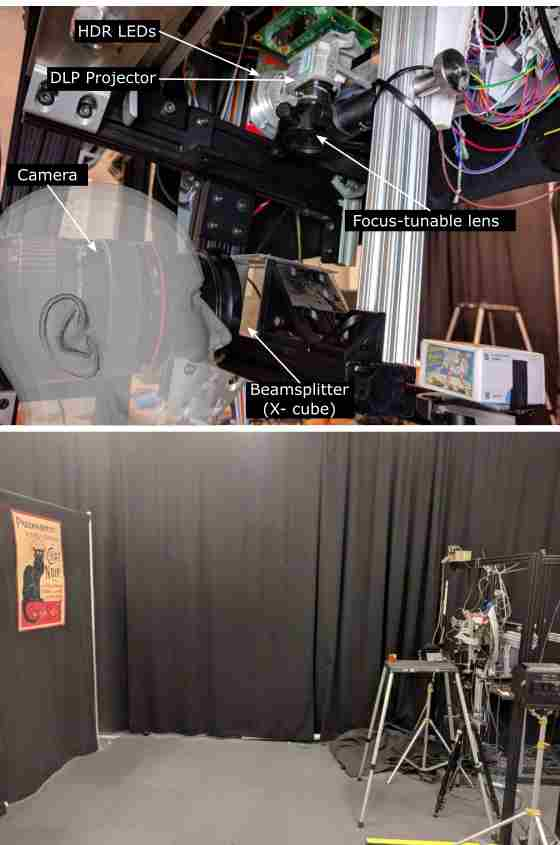
\includegraphics[width=0.8\columnwidth]{images/volumetric/setup}
\caption[Volumetric NED: prototype and staged real-world scene for capturing results]{\emph{Top:} Our prototype display. \emph{Bottom:} The staged real-world scene used to collect all see-through images and videos. Multiple objects (a tiny rubber ducky (2cm height), a wristwatch, a Rubik's cube, and a wall poster) are arranged progressively from near to far. Virtual objects are rendered in this staged real-world scene such that each virtual object is located at the same depth as one of the real world objects (See Figure~\ref{fig:volumetric:results}).}
\label{fig:volumetric:setup}
\end{figure}



\paragraph{Optics} Other than the focus-tunable lens, we use the manufacturer-provided optical engine of the TI Discovery 4100 Kit (STAR-07 optical module), a Fresnel lens (60mm focal length), and a beamsplitter that allows the display to optically integrate the real world view and the imagery of the virtual scene. 

\paragraph{DMD controller} 
The DMD controller we use is the Texas Instruments (TI) Digital Light Processing (DLP) Discovery 4100 Kit which drives an XGA (1024 x 768) DMD module. The display system is capable of displaying binary images at up to 17241 Hz which would allow 287 binary images to be displayed in each lens cycle. This would need precise synchronization between the lens signal and the DMD controller, which is not afforded by the current implementation. For a more robust system, we display 280 images in each lens cycle and design the system such that the 280 images are guaranteed to be displayed slightly before the beginning of the next lens cycle. 

\paragraph{Custom RGB LED Illuminator}
A PCB mounted RGB LED is controlled using electronics consisting of Digital-Analog-Converters (DACs), Op-Amps, etc. The board listens for three 16-bit binary codes over Serial Peripheral Interface (SPI) protocol over three parallel buses and sets each color LED to the brightness level corresponding to the received code. The board is capable of illuminating the DMD with a wide range of brightnesses and color combinations. $2^{16}$ levels of intensity are possible for each color LED and all color LEDs can be driven in parallel. The full-scale rise and fall times of each channel are approximately 500ns; every binary frame can be illuminated at a distinct intensity and color mix. This RGB LED illuminator is the same as the one used in Lincoln et al.~\cite{Lincoln2017scene}; please refer to that chapter for more details. 

\paragraph{PC}
A PC using Intel Xeon E5-2630 2.4 GHz processor with an NVIDIA GeForce GTX 980 running Windows 7 is used to implement an offline version of the proposed rendering pipeline. 


\subsection{Operational detail}
Figure~\ref{fig:volumetric:blockdiagram-timing} gives an overview of the operation of the NED. The binary images are uploaded to the DMD controller using the ALP 4.1 Controller Suite. The DMD controller is configured to advance frames each time it receives a trigger signal from the microcontroller. At the end of the sequence of images, the DMD cycles back to the first image. The frametime of the DMD was set to the minimum possible frametime of 58 $\mu s$.

The lens controller outputs a trigger signal whose rising edges correspond to the beginning of each lens's cycle. The lens operates at a frequency of 60 Hz. The lens' trigger signal is detected by the microcontroller, which then performs $280$ instances of these operations before the next lens' trigger signal: (1) microcontroller outputs a trigger signal to the DMD controller, and (2) microcontroller sends three 16-bit words to the LED controller. Each 16-bit word specifies the brightness of a color LED. The microcontroller ensures that the DMD updates and illumination values are phase-locked to the lens cycle. Figure~\ref{fig:volumetric:setup} shows an image of our display's hardware and the experimental setup. 

\subsubsection{Calibrating phase delay}
In our experience, we've found that there is a phase delay between the lens signal and the displayed image plane depth estimated in Figure~\ref{fig:volumetric:graphs}. This phase delay was calibrated visually by generating a synthetic stack of images in which each image has a single feature (like a cross-hair), but the feature is placed at a different location in each image. By setting the camera lens to nearest focus, it was visually determined that the $180$th image out of the $280$ image stack is in focus, which meant that the lens trigger signal and our system's display of the virtual images are out of phase by $\frac{180 - 140}{280} \times 16.67ms = 2.38 ms$. To correct for this, the binary images uploaded to the DMD controller were cyclically rearranged such that the $180$th binary image is moved to the $140$th index.

\subsection{Future implementation improvements}
The results can be visually improved by performing white-balance correction, gamma curve calibration, and calibrating for the non-uniform frustum as shown in the last row of Figure~\ref{fig:volumetric:graphs}. In our experience, we didn't find the change in FoV to reduce the image quality significantly, but it does make long straight objects slightly curved, especially when the straight objects are places towards the periphery of the display. 

